\documentclass{article}
\usepackage{amsmath,amssymb,amsbsy}
\usepackage{graphicx}
\usepackage[letterpaper,lmargin=2.5cm,rmargin=2.5cm,tmargin=2.5cm,bmargin=2.5cm]{geometry}
\usepackage{color}
\usepackage{listings}
\usepackage{float}
\usepackage{listings-python-options}
\usepackage{graphicx,caption,subcaption}
% some useful definitions:

\newcommand{\tr}{\intercal} % transpose
% we use boldface math characters often so let's create some shortcuts:
\newcommand{\X}{\mathbf{X}}
\newcommand{\x}{\mathbf{x}}
\newcommand{\y}{\mathbf{y}}
\newcommand{\w}{\mathbf{w}}
% some useful operators
\newcommand{\argmax}[1]{\underset{#1}{\operatorname{argmax}}}
\newcommand{\argmin}[1]{\underset{#1}{\operatorname{argmin}}}



\begin{document}

\title{CS545 Machine Learning - Assignment 4}
\author{Yu, Qiu}
\maketitle

\noindent\hrulefill
\vspace{-5mm} %to remove some whitespace before "Contents"
\tableofcontents
\noindent\hrulefill

\section{Part 1: Activation Functions}
\subsection{Formula Derivation}
\begin{enumerate}
	\item Recall that:
	\begin{align}
	\sigma(x)& = \frac{1}{1+exp(-x)}\\
	\end{align}
	So, \\
	\begin{align}
	\sigma(x)+\sigma(-x) &=\frac{1}{1+e^{-x}}+\frac{1}{1+e^{x}}\\
	&=\frac{(1+e^{x})+(1+e^{-x})}{(1+e^{-x})(1+e^{x})}\\
	&=\frac{2+e^{x}+e^{-x}}{1+e^{-x}+e^{x}+1}\\
	&=1
	\end{align}
	Therefore,
	\begin{align}
	\sigma(x) + \sigma(-x) &= 1\\
	\sigma(x) = 1 - \sigma(-x)
	\end{align}
	\item 
	\begin{align}
	2\sigma(2x)-1 &= \frac{2}{1+e^{-2x}}-1\\
	&=\frac{2-1-e^{-2x}}{1+e^{-2x}}\\
	&=\frac{1-e^{-2x}}{1+e^{-2x}}\\
	&=\frac{e^{-x}(e^{x}-e^{-x}}{e^{-x}(e^{x}+e^{-x})}\\
	&=\frac{e^{x}-e{-x}}{e^{x}+e{-x}}\\
	\end{align}
	Recall that:\\
	\begin{align}
	tanh(x) = \frac{exp(x)-exp(-x)}{exp(x)+exp(-x)}
	\end{align}
	So,
	\begin{align}
	tanh(x) = 2\sigma(2x)-1
	\end{align}
	\end{enumerate}
\subsection{Equivalent Network}
	According to the textbook 7.3, for a single hidden layer, the formula to get the prediction for the output layer is:
	\begin{align}
	h(x) = \theta\left(w_{01}^{(2)}+\sum_{j=1}^{m}w_{j1}^{(2)}\cdot tanh(\sum_{i=0}^{d}w_{ij}^{(1)}x_{i})\right)
	\end{align}
	Applying formula (16), then we got:
	\begin{align}
		h(x) &= \theta\left(w_{01}^{(2)}+\sum_{j=1}^{m}w_{j1}^{(2)}\cdot tanh(\sum_{i=0}^{d}w_{ij}^{(1)}x_{i})\right)\\
		h(x) &= \theta\left(w_{01}^{(2)}+\sum_{j=1}^{m}w_{j1}^{(2)}\cdot \left(2\sigma(2\sum_{i=0}^{d}w_{ij}^{(1)}x_{i})-1\right)\right)\\
		h(x) &= \theta\left(w_{01}^{(2)}+2\sum_{j=1}^{m}w_{j1}^{(2)}\cdot \sigma(\sum_{i=0}^{d}2w_{ij}^{(1)}x_{i})-\sum_{j=1}^{m}w_{j1}^{(2)}\right)\\
		h(x) &= \theta\left(\left(w_{01}^{(2)}-\sum_{j=1}^{m}w_{j1}^{(2)}\right)+2\sum_{j=1}^{m}w_{j1}^{(2)}\cdot \sigma(\sum_{i=0}^{d}2w_{ij}^{(1)}x_{i})\right)
	\end{align}
	Let:
	\begin{align}
	v_{01}^{(2)} &= w_{01}^{(2)}-\sum_{j=1}^{m}w_{j1}^{(2)}, \quad j =(1,2,...,m)\\
	v_{j1}^{(2)} &= 2w_{ji}^{(2)},\quad j=(1,2,...,m)\\
	v_{ij}^{(1)} &= 2w_{ij}^{(1)},\quad i=(1,2,...,d) \quad j =(1,2,...,m)
	\end{align}
	Then:
	\begin{align}
		h(x) = \theta\left(v_{01}^{(2)} +\sum_{j=1}^{m}v_{j1}^{(2)}\cdot \sigma(\sum_{i=0}^{d}v_{ij}^{(1)}x_{i})\right)
	\end{align}
	Therefore, if we replace old weight vector $w_{ij}$ with the new weight vector $v_{ij}$ from formula $(22) \sim (24)$, we can get the result which applied logistic sigmod as activation function. 
	
\section{Multi-layer perceptrons}
For the following decision boundary, we assign 4 functions to each line: h1, h2, h3, h4.
\begin{figure}[H]
	\centering
	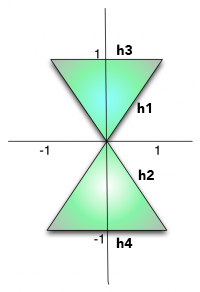
\includegraphics[width = 2in]{figure/boundary.png}
	\caption{Decision Boundary}
\end{figure}
In order to achieve the specified area, we noticed that the area is alway at bottom of h3, on top of h4. For h1 and h2, the area is always at the same side of h1 and h2. More specifically, for any point $(x, y)$ in the area, $sign(h1(x))=sign(h2(x))$. So the multilayer perceptron implementation should be:
\begin{align}
f(x)=h1\cdot h2\cdot \overline{h3}\cdot h4+\overline{h1}\cdot \overline{h2}\cdot\overline{h3}\cdot h4
\end{align}
\section{Exploring neural networks for digit classification}
\subsection{Add Bias Term}
First of all, the given implementation does not provide bias term correctly. In the given code:
\begin{lstlisting}
def forward(self, x) :
    a = [x]
    for i in range(self.num_layers) :
	    a.append(self.activation(np.dot(a[i], self.weights[i])))
    return a
\end{lstlisting}
It only applies bias term for the input layer correctly, but for the hidden layer, it computes the bias term $w_{0}$ based on the previous result, which is not right. So we have to modify it in order to get the correct bias term:
\begin{lstlisting}
def forward(self, x):
    a = [x]
    for i in range(self.num_layers):
	    ai = self.activation(np.dot(a[i], self.weights[i]))
	    if (len(a) < self.num_layers):
		    ai[-1] = 1
		a.append(ai)
    return a
\end{lstlisting}

\subsection{Single hidden layer neural network}
For single hidden layer neural network, we first modified test\_digits method, so that it can get the accuracy from confusion matrix:
\begin{lstlisting}
def test_digits_single_hidden_layer(hidden_layer_units):
	digits = load_digits()
	X = digits.data
	y = digits.target
	X /= X.max()  # Normalize data
	
	nn = NeuralNetwork([64, hidden_layer_units, 10], 'logistic')
	X_train, X_test, y_train, y_test = train_test_split(X, y, 
								test_size=0.25, random_state=0)
	labels_train = LabelBinarizer().fit_transform(y_train)
	labels_test = LabelBinarizer().fit_transform(y_test)
	nn.fit(X_train, labels_train, epochs=100)
	predictions = []
	for i in range(X_test.shape[0]):
		o = nn.predict(X_test[i])
		predictions.append(np.argmax(o))
	cm = confusion_matrix(y_test, predictions)
	correct_prediction = 0.0
	for i in range(cm.shape[0]):
		correct_prediction += cm[i][i]
	accuracy = correct_prediction / X_test.shape[0]
	return accuracy
\end{lstlisting}

Then in order to plot the graph between accuracy and the number of hidden layer units, we have to use a loop to calculate accuracy under different number of hidden layer units. For speed purpose, we step 10\% of current units number:
\begin{lstlisting}
max_hidden_layer_units_1 = 1000
## single hidden layer
unit_1 = 1
units_1 = []
accuracy_1 = []
while unit_1 <= max_hidden_layer_units_1:
	units_1.append(unit_1)
	unit_1 += math.ceil(unit_1 / 10)
units_1 = units_1[1:]
for unit in units_1:
	accuracy_1.append(test_digits_single_hidden_layer(unit))

plt_units = np.asarray(units_1)
plt_accuracy = np.asarray(accuracy_1)
plt.plot(plt_units, plt_accuracy, "b")
plt.xlabel("Hidden Layer Units")
plt.ylabel("Accuracy")
plt.show()
\end{lstlisting}

Below is the graph we got:
 \begin{figure}[H]
 	\centering
 	\begin{subfigure}{.45\textwidth}
 		\centering
 		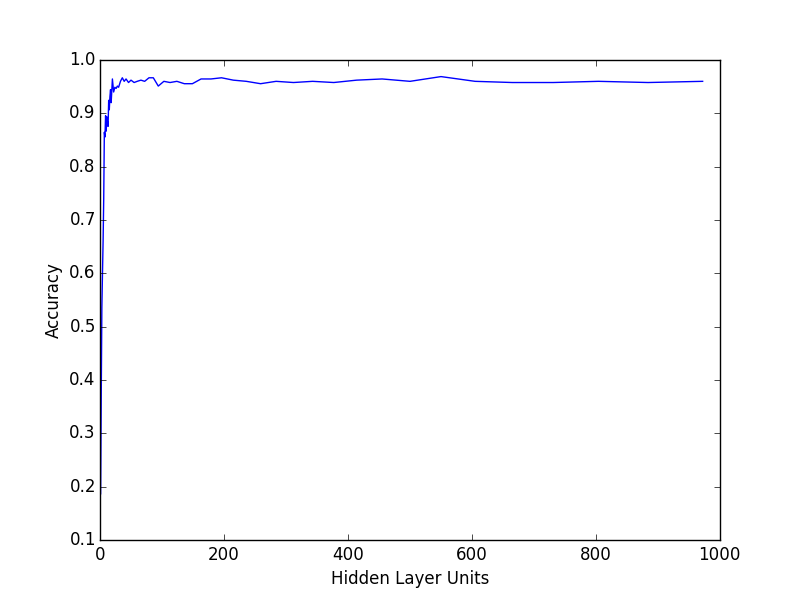
\includegraphics[width=2in]{figure/figure_1.png}
 	\end{subfigure}
 	\begin{subfigure}{.45\textwidth}
 		\centering
 		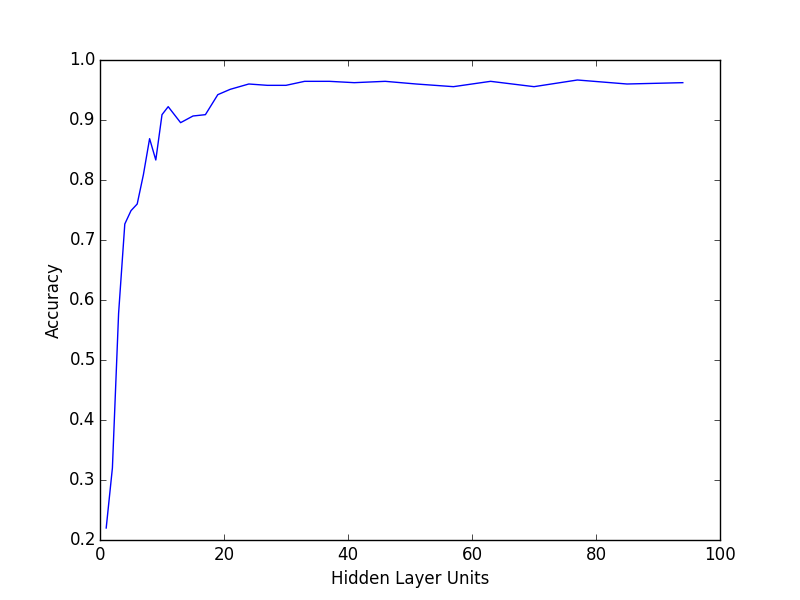
\includegraphics[width=2in]{figure/figure_1_2.png}
 	\end{subfigure}
 \end{figure}
As we can see, the relation between hidden layer units and accuracy is almost linear when units is relatively small, say less than 100, where underfitting happens. While when the hidden layer units is larger, the accuracy stays at a high level. For this dataset, overfitting is quite hard to happen.
\subsection{Two hidden layers neural network}
In order to add an additional layer to the neural network, we have to slightly modify the test\_digits method again:
\begin{lstlisting}
def test_digits_two_hidden_layers(hidden_layer1_units, hidden_layer2_units):
	digits = load_digits()
	X = digits.data
	y = digits.target
	X /= X.max()  # Normalize data
	
	nn = NeuralNetwork([64, hidden_layer1_units, hidden_layer2_units, 10], 'logistic')
	X_train, X_test, y_train, y_test = train_test_split(X, y, 
								test_size=0.25, random_state=0)
	labels_train = LabelBinarizer().fit_transform(y_train)
	labels_test = LabelBinarizer().fit_transform(y_test)
	nn.fit(X_train, labels_train, epochs=100)
	predictions = []
	for i in range(X_test.shape[0]):
		o = nn.predict(X_test[i])
		predictions.append(np.argmax(o))
	cm = confusion_matrix(y_test, predictions)
	correct_prediction = 0.0
	for i in range(cm.shape[0]):
		correct_prediction += cm[i][i]
	accuracy = correct_prediction / X_test.shape[0]
	print accuracy
	return accuracy
\end{lstlisting}
Then we use two loops to get the relationship between accuracy and number of both hidden layer units:
\begin{lstlisting}
max_hidden_layer_units_2 = 200
unit_2 = 1
units_2 = []
accuracy_2 = []
while unit_2 <= max_hidden_layer_units_2:
	units_2.append(unit_2)
	unit_2 += math.ceil(unit_2 / 10)
units_2 = units_2[1:]
accuracy_mat_2 = np.zeros((len(units_2), len(units_2)))

for i in range(len(units_2)):
	for j in range(len(units_2)):
		accuracy_mat_2[i][j] = test_digits_two_hidden_layers(units_2[i], units_2[j])

plt_units_1 = np.asarray(units_2)
plt_units_2 = np.asarray(units_2)
plt.pcolor(plt_units_1, plt_units_2, accuracy_mat_2, cmap='gnuplot')
plt.xlabel("Hidden Layer 1 Units")
plt.ylabel("Hidden Layer 2 Units")
plt.colorbar()
plt.show()
\end{lstlisting}
Here is the figure we got:
 \begin{figure}[H]
 	\centering
	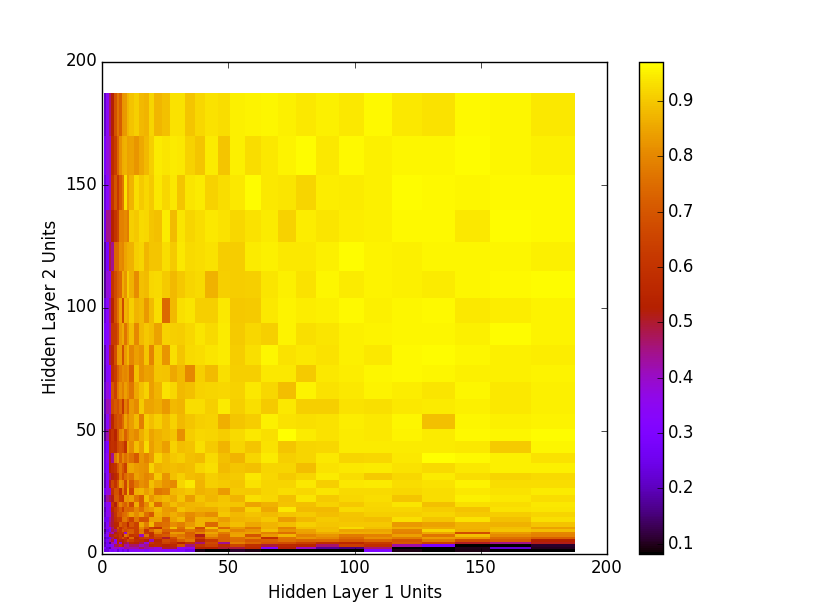
\includegraphics[width=3in]{figure/figure_2_2.png}
 \end{figure}
From the figure above, we can see that when either one of the hidden layer has few units, the accuracy will be relatively low. When both hidden layer increase their units number, the accuracy increases dramatically. More specifically, when hidden layer units are under 50, the accuracy are normally below 80\%, which is underfitting. And when both layer units are more than 50, the accuracy keeps at a high level, generally more than 90\%. 

\subsection{Weight Decay}
According to the chapter 7.4.1 on textbook, in order to add a weight decay term, we need to modify the error total as below:
\begin{align}
E_{aug}(\mathbf{w})&=E_{in}(\mathbf{w})+\frac{\lambda}{N}\sum_{l,i,j}(w_{ij}^{(l)})^{2}\\
\frac{\partial E_{aug}(\mathbf{w})}{\partial \mathbf{W}^{(l)}}&=\frac{E_{in}(\mathbf{w})}{\partial \mathbf{W}^{(l)}}+\frac{2\lambda}{N}\mathbf{W}^{(l)}
\end{align}
So we need to modify given code at fit method:
\begin{lstlisting}
def fit(self, X, y, learning_rate=0.2, epochs=50, _lambda=0.0, linear=False):
	X = np.asarray(X)
	temp = np.ones((X.shape[0], X.shape[1] + 1))
	temp[:, 0:-1] = X  # adding the bias unit to the input layer
	X = temp
	y = np.asarray(y)
	
	for k in range(epochs):
		I = np.random.permutation(X.shape[0])
		for i in I:
			a = self.forward(X[i], linear)
			deltas = self.backward(y[i], a, linear)
			# update the weights using the activations and deltas:
			for i in range(len(self.weights)):
				layer = np.atleast_2d(a[i])
				delta = np.atleast_2d(deltas[i])
				N = len(a[-1])
				self.weights[i] += learning_rate * (layer.T.dot(delta) + _lambda / N * self.weights[i])
\end{lstlisting}
We modified the last line, where the weight vector got updated:
\begin{lstlisting}
self.weights[i] += learning_rate * (layer.T.dot(delta) + _lambda / N * self.weights[i])
\end{lstlisting}
And we got the following figures:
 \begin{figure}[H]
 	\centering
 	\begin{subfigure}{.45\textwidth}
 		\centering
 		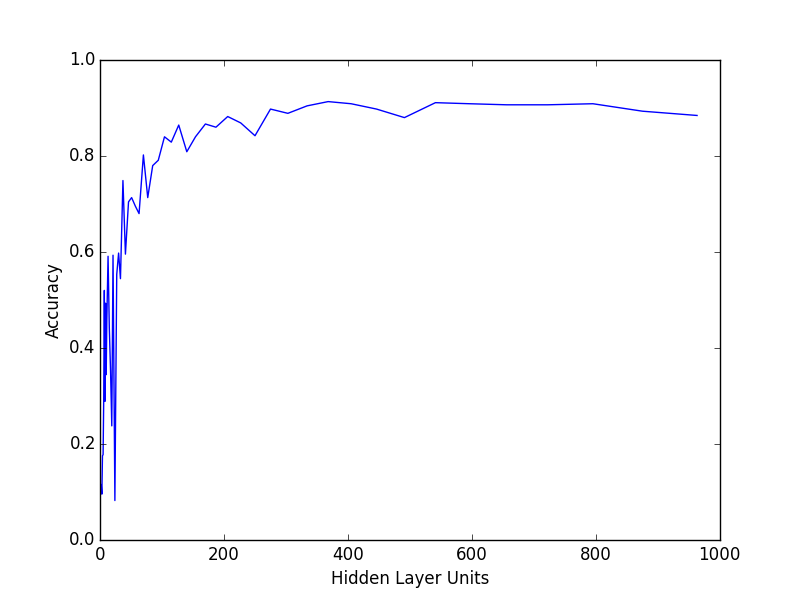
\includegraphics[width=2in]{figure/figure_3.png}
 	\end{subfigure}
 	\begin{subfigure}{.45\textwidth}
 		\centering
 		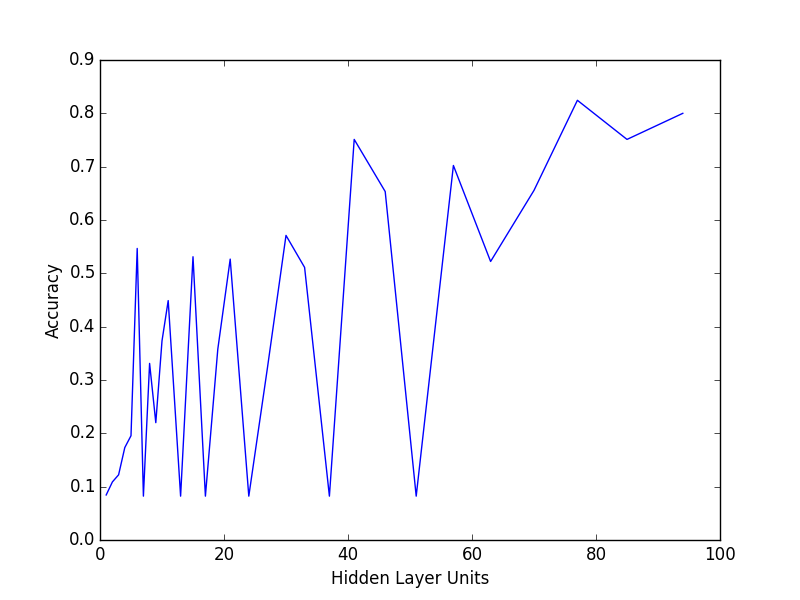
\includegraphics[width=2in]{figure/figure_3_2.png}
 	\end{subfigure}
 \end{figure}
We found that the accuracy performed worse than that without weight decay term. That is because the weight decay method is used for avoid overfitting situation. However, the given dataset is very well built, and it hardly has overfitting problem. We increased the hidden layer units number to 10000 but there is still no overfitting. Therefore, if we apply weight decay term, it will have an underfitting problem for this specific dataset.

\subsection{Linear Activation Function}
Normally, in a nerual network we offen use sigmod function as activation function, while in output layer, we often use a linear function. This is because that the sigmod function will only output values between 0 to 1. However, in the output layer, we have to compare the outputs to label y. A linear function can scale the output to arbitrary value, which is better for the comparison purpose. \\
\\
We need to modify the code accordingly in order to apply linear activation function at output layer: If the layer is the last layer, we will apply linear function: $f=x$.

\begin{lstlisting}
def forward(self, x, linear=False):
	a = [x]
	for i in range(self.num_layers):
		ai = self.activation(np.dot(a[i], self.weights[i]))
		if i == self.num_layers - 1 and linear == True:
			ai = np.dot(a[i], self.weights[i])
		if (len(a) < self.num_layers):
			ai[-1] = 1
		a.append(ai)
	return a
\end{lstlisting}
\begin{lstlisting}
def backward(self, y, a, linear=False):
	if linear:
		deltas = [(y - a[-1])] * 1
	else:
		deltas = [(y - a[-1]) * self.activation_deriv(a[-1])]
	for l in range(len(a) - 2, 0, -1):  # we need to begin at the second to last layer
		deltas.append(deltas[-1].dot(self.weights[l].T) * self.activation_deriv(a[l]))
	deltas.reverse()
	return deltas
\end{lstlisting}

And we got the following graph:
\begin{figure}[H]
\centering
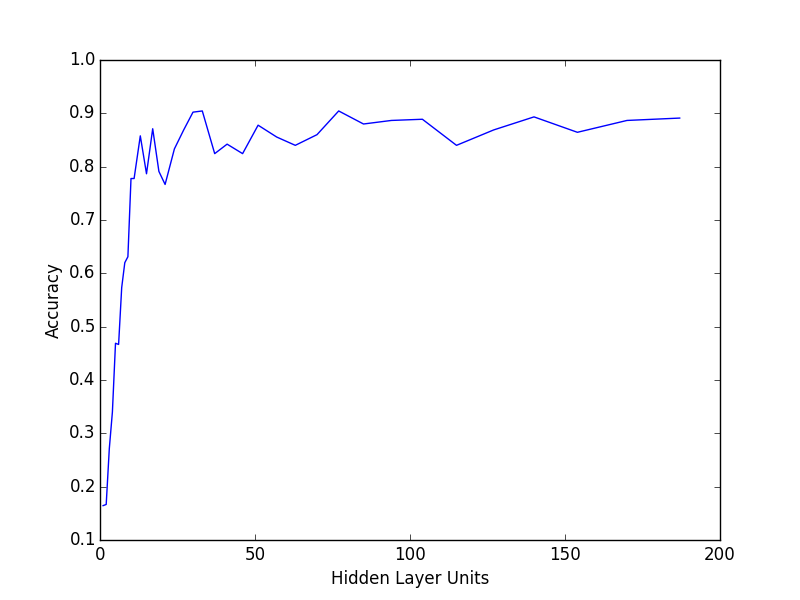
\includegraphics[width=3in]{figure/figure_4_2.png}
\end{figure}

\bibliography{start.bib}
\bibliographystyle{plain}

\end{document}
